\documentclass[fleqn]{slnotes}
\usepackage{wrapfig}

\setlength{\mathindent}{0pt}
\DeclareMathOperator{\Exists}{\exists}
\DeclareMathOperator{\Forall}{\forall}

\begin{document}
\chapter{CS3230: Mathematics}

\sldef{Arithmetic series}. \begin{align*}
\sum^n_{k=1} k &= \frac{1}{2}n(n+1) = \Theta(n^2)\\
\sum^n_{k=0} k^2 &= \frac{1}{6}n(n+1)(2n+1) = \Theta(n^3)\\
\sum^n_{k=0} k^3 &= \frac{1}{4}n^2{(n+1)}^2 = \Theta(n^4)
\end{align*}

\sldef{Geometric series}. \begin{align*}
\sum^n_{k=0}x^k &= \frac{x^{n+1}-1}{x-1}\\
\sum^\infty_{k=0}x^k &= \frac{1}{1-x}\quad\left(\left|x\right| < 1\right)
\end{align*}

\sldef{Harmonic series}. \begin{align*}
H_n = \sum^n_{k=1}\frac{1}{k} = \ln n + O(1)
\end{align*}

\sldef{Logarithms}. \begin{align*}
\lg_b a &= 1/(\lg_a b)\\
\lg^k n &= {(\lg n)}^k\\
\lg \lg n &= \lg (\lg n)
\end{align*}

\sldef{L'Hopital's rule}. \begin{align*}
\lim_{x\to\infty}\frac{f(x)}{g(x)} &= \lim_{x\to\infty}\frac{f'(x)}{g'(x)}
\end{align*}

\sldef{Stirling's approximation}. \begin{align*}
\lg n! = \Theta(n \lg n)
\end{align*}

\sldef{Limits}. \begin{align*}
\lim_{n\to\infty}\frac{f(n)}{g(n)} = 0 &\Rightarrow f(n) \in o(g(n))\\
\lim_{n\to\infty}\frac{f(n)}{g(n)} < \infty &\Rightarrow f(n) \in O(g(n))\\
0 < \lim_{n\to\infty}\frac{f(n)}{g(n)} < \infty &\Rightarrow f(n) \in \Theta(g(n))\\
\lim_{n\to\infty}\frac{f(n)}{g(n)} > 0 &\Rightarrow f(n) \in \Omega(g(n))\\
\lim_{n\to\infty}\frac{f(n)}{g(n)} = \infty &\Rightarrow f(n) \in \omega(g(n))
\end{align*}

\sldef{Asymptotic notation}. \begin{align*}
O(g(n)) &= \{ f(n) \mid \Exists c > 0, n_0 > 0 \\
        &: 0 \le f(n) \le c g(n) \Forall n \ge n_0 \}\\
\Omega(g(n)) &= \{ f(n) \mid \Exists c > 0, n_0 > 0 \\
             &: 0 \le c g(n) \le f(n) \Forall n \ge n_0 \}\\
\Theta(g(n)) &= \{ f(n) \mid \Exists c_1 > 0, c_2 > 0, n_0 > 0 \\
             &: 0 \le c_1 g(n) \le f(n) \le c_2 g(n) \Forall n \ge n_0 \}\\
             &= O(g(n)) \cap \Omega(g(n))\\
o(g(n)) &= \{ f(n) \mid \Forall c > 0, \Exists n_0 > 0 \\
        &: 0 \le f(n) < c g(n) \Forall n \ge n_0 \}\\
\omega(g(n)) &= \{ f(n) \mid \Forall c > 0, \Exists n_0 > 0 \\
        &: 0 \le c g(n) < f(n) \Forall n \ge n_0 \}
\end{align*}

\(O \approx \mathord{\le}\). \(\Omega \approx \mathord{\ge}\). \(o \approx \mathord{<}\). \(\omega \approx \mathord{>}\).

\sldef{Properties of asymptotic notation}. \begin{align*}
\Forall &X \in \{o,O,\Theta,\Omega,\omega\}, \text{(Transitivity)}\\
  &f(n) \in X(g(n)) \land g(n) \in X(h(n)) \Rightarrow f(n) \in X(h(n))\\
\Forall &X \in \{O,\Theta,\Omega\}, \text{(Reflexivity)}\\
  &f(n) \in X(f(n))\\
\intertext{(Complementarity)}
&f(n) \in O(g(n)) \Leftrightarrow g(n) \in \Omega(f(n))\\
&f(n) \in o(g(n)) \Leftrightarrow g(n) \in \omega(f(n))\\
\intertext{Symmetry}
&f(n) \in \Theta(g(n)) \Leftrightarrow g(n) \in \Theta(f(n))
\end{align*}

\sldef{Common relations}. For constant \(a > 1\), \[
\lg n \ll \lg^a n \ll n \ll n^a \ll a^n \ll n! \ll n^n
\]

\sldef{Master theorem}.
\begin{gather*}
\text{For } T(n) = aT\left(\frac{n}{b}\right) + \Theta(f(n)),\\
\text{1. } f(n) \in O(n^{(\log_b a)-\epsilon}), \epsilon > 0 \Rightarrow T(n) \in \Theta(n^{\log_b a})\\
\text{2. } f(n) \in \Theta(n^{\log_b a} \lg^k n), k \ge 0 \Rightarrow T(n) \in \Theta(f(n) \lg n)\\
\text{3. } f(n) \in \Omega(n^{(\log_b a) + \epsilon}), \epsilon > 0 \land a f\left(\frac{n}{b}\right) \le c f(n), c < 1\\
\quad \Rightarrow T(n) \in \Theta(f(n))
\end{gather*}

\sldef{Triangle numbers}. \(a_n = \frac{1}{2}n(n+1)\), also the sum of the first \(n\) natural numbers, and the sum of two consecutive terms is a square number.

\sldef{Fibonacci}. \(\forall n \in \mathbb{N}, F_0 = 0, F_1 = 1, F_n = F_{n-1} + F_{n-2} = \frac{1}{\sqrt 5}(\phi^n - (-\phi)^{-n})\) where \(\phi = \frac{1}{2}(1 + \sqrt5)\).

A recurrence relation \(a_k = Aa_{k-1} + Ba_{k-2}\) for all integers \(k \ge 2\) is satisfied by the sequence \(1, t, t^2, t^3, \hdots\) where \(t\) is a nonzero real number iff \(t\) satisfies the characteristic equation \(t^2 - At - B = 0\).

\sldef{Distinct roots theorem}. If a recurrence relation \(a_k = Aa_{k-1} + Ba_{k-2}\), \(B \neq 0\) for all integers \(k \ge 2\) has a characteristic equation \(t^2 - At - B = 0\) with two distinct roots \(r\) and \(s\), then the explicit formula is \(a_k = Cr^n + Ds^n\), with the values of \(C\) and \(D\) being determined by \(a_0\) and \(a_1\).

If a recurrence relation \(a_k = Aa_{k-1} + Ba_{k-2}\) for all integers \(k \ge 2\) has a characteristic equation \(t^2 - At - B = 0\) with one repeated root \(r\), then the sequences \(1, r, r^2, r^3, \hdots\) and \(0, r, 2r^2, 3r^3, \hdots\) both satisfy the recurrence relation for all integers \(k \ge 2\).

\sldef{Single root theorem}. If a recurrence relation \(a_k = Aa_{k-1} + Ba_{k-2}\), \(B \neq 0\) for all integers \(k \ge 2\) has a characteristic equation \(t^2 - At - B = 0\) with one repeated root \(r\), then the explicit formula is \(a_k = Cr^n + Dnr^n\), with the values of \(C\) and \(D\) being determined by \(a_0\) and \(a_1\).

\chapter{Correctness}
\sldef{\dots of iterative algorithms}. Find an \sldef{invariant} which is true at the beginning of every iteration. Prove (by induction) that the invariant is true before the first iteration (\sldef{initialisation}), that if it is true at the start of one iteration, it remains true at the start of the next (\sldef{maintenance}), and that the invariant somehow proves the correct result at the end (\sldef{termination}).

\chapter{Divide-and-conquer algorithms}
\sldef{Merge sort}. Divide array into half. Recursively sort two halves. Merge in linear-time. \(\Theta(n \lg n)\).

\sldef{Binary search}. Check middle element. Recursively search one array, if needed. \(\Theta(\lg n)\).

\sldef{Exponentiation}. Recurse by halving the exponent and squaring the result. \(\Theta(\lg n)\).

\sldef{Computing Fibonacci}. \(\Theta(\lg n)\). Reduce to: \[
\begin{bmatrix}
F_{n+1} & F_n\\
F_n & F_{n-1}
\end{bmatrix}
=
\begin{bmatrix}
1&1\\1&0
\end{bmatrix}^n
\]

\sldef{Strassen's matrix multiplication}. \(\Theta(n^{\lg 7})\). Divide the input matrices into 4 quarters each. Create 10 matrices from the sum or difference of two matrices from the previous step. Recursively compute seven (this is what makes this faster than \(\Theta(n^3)\)) matrix products. Compute the submatrices of the result matrix C by adding and subtracting combinations of the result from the previous step.

\sldef{H-tree embedding}. \(\Theta(n)\) area. 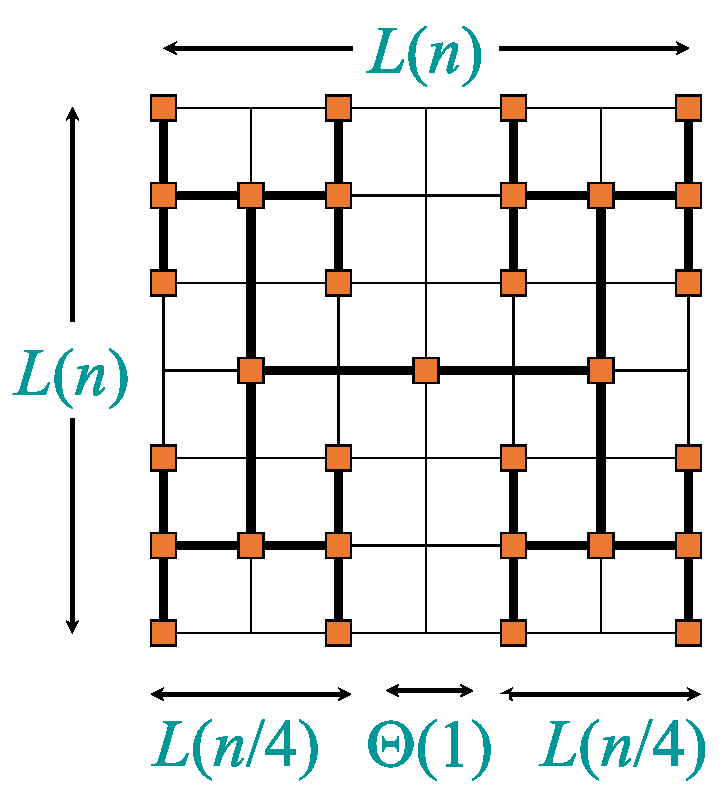
\includegraphics[width=0.3\columnwidth]{htree-embedding.pdf}

\chapter{Sorting}
\sldef{Lower bound for comparison-based sorting}. \(\Omega(n \lg n)\) comparisons.

\sldef{Counting sort}. Stable, not in-place. \(\Theta(n+k)\), for \(n\) input integers 0 to \(k\).\\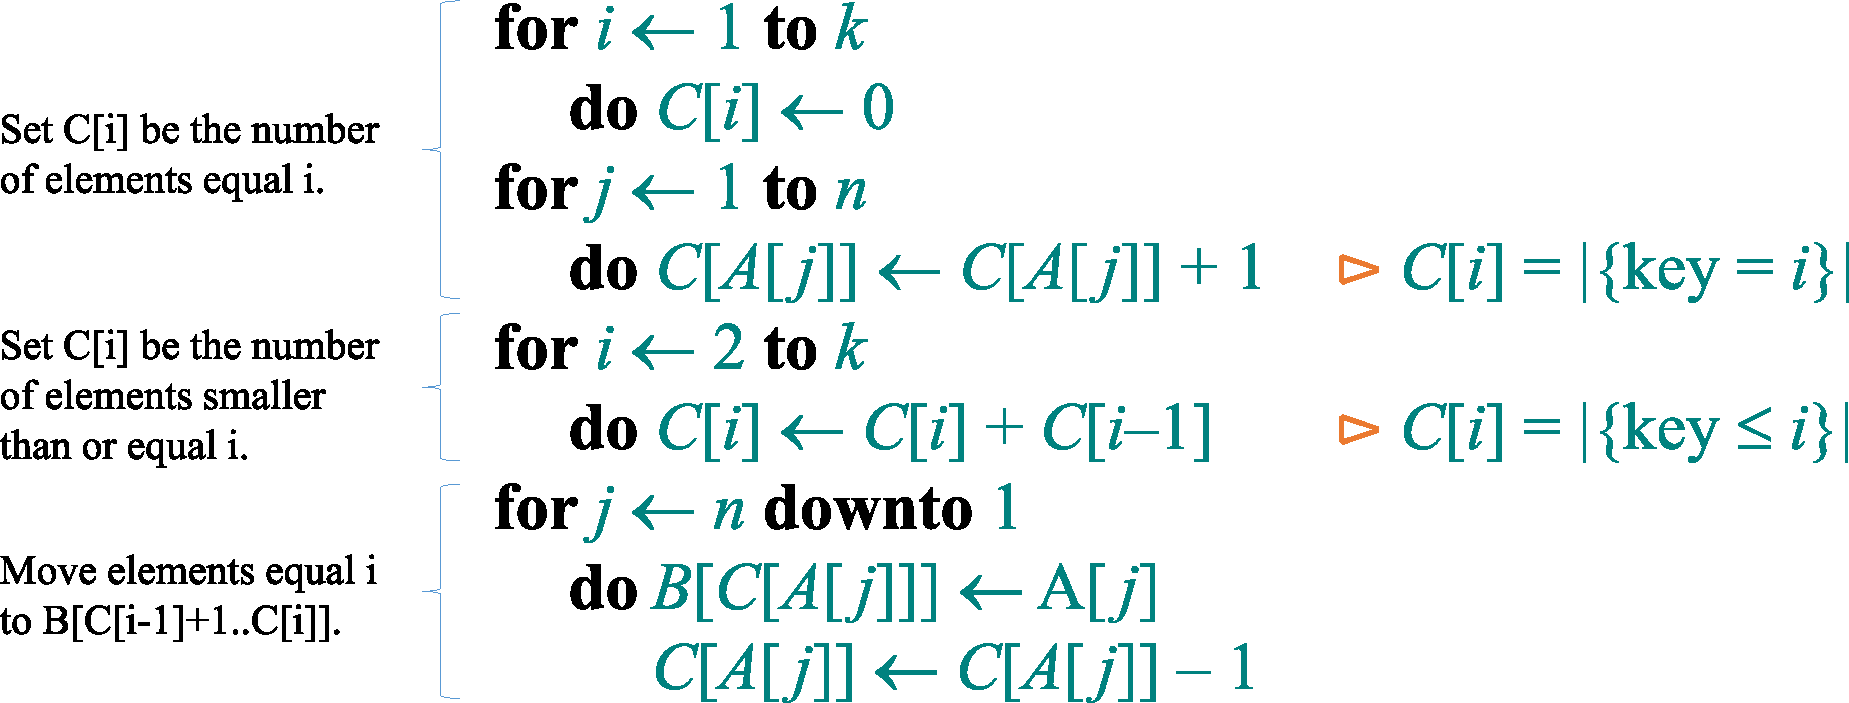
\includegraphics[width=\columnwidth]{counting-sort.pdf}

\sldef{Radix sort}. Sort by digits, from least significant, using a stable sort (e.g. counting). \(T(n,b) = \Theta((b/r)(n+2^r))\), to sort \(n\) \(b\)-bit numbers from 1 to \(k\) by breaking them up into \(r\)-bit pieces. Optimal \(r\) is slghtly smaller than \(\lg n\). \(r = \lg n\) implies \(T(n, b) = \Theta(bn/\lg n)\).

\sldef{Sort summary}.

\begin{tabular}{lllll}
\toprule
Sort & St & IP & Ave. & Worst \tabularnewline
\midrule
Quick & N & Y & \(O(n \lg n)\) & \(O(n^2)\) \tabularnewline
Merge & Y & N & \(O(n \lg n)\) & \(O(n \lg n)\) \tabularnewline
Heap & N & Y & \(O(n \lg n)\) & \(O(n \lg n)\) \tabularnewline
Insertion & Y & Y & \(O(n^2)\) & \(O(n^2)\) \tabularnewline
Selection & N* & Y & \(O(n^2)\) & \(O(n^2)\) \tabularnewline
Bubble & Y & Y & \(O(n^2)\) & \(O(n^2)\) \tabularnewline
\bottomrule
\end{tabular}

\chapter{Randomized algorithms}
\sldef{Monte Carlo}. Runtime is independent of randomness, but gives only an approximate answer.

\sldef{Las Vegas}. Always gives the correct answer, but runtime depends on randomness.

\sldef{Probability}.
\begin{gather*}
P(A \cup B) = P(A) + P(B) - P(A \cap B)\\
P(A \cap B) = P(A) \cdot P(B) \Leftrightarrow \text{independent}\\
P(A \mid B) = P(A \cap B) / P(B) = P(A)P(B\mid A)/ P(B)\\
= P(A)P(B\mid A)/(P(A)P(B\mid A) + P(A')P(B\mid A'))\\
E[X] = \sum_x x\cdot P(X = x)\\
E[X+Y] = E[X] + E[Y]\\
E[XY] = E[X]E[Y] \text{ if independent}
\end{gather*}

\sldef{Bernoulli trial}. Such a trial has probability \(p\) of success and \(q = 1 - p\) of failure.

\sldef{Geometric distribution}. If we have a sequence of independent Bernoulli trials of probability-\(p\) success, and \(X\) is the number of trials needed to obtain success for the first time, then \(X\) follows the geometric distribution. \begin{gather*}
P(X = k) = q^{k-1}p\quad E[X] = 1/p
\end{gather*}

\sldef{Binomial distribution}. Let \(X\) be the number of successes in \(n\) Bernoulli trials. Then \(X\) follows the binomial distribution. \begin{gather*}
P(X = k) = \binom{n}{k}p^k q^{n-k} \quad E[X] = np
\end{gather*}

\sldef{Indicator variable}. An indicator variable \(I_A\) for an event \(A\) is 1 if \(A\) occurs, and \(0\) otherwise. Importantly, \begin{gather*}
E[I_A] = P(A)
\end{gather*}

\sldef{Coupon collecting}. There are \(n\) types of coupon to be collected. Coupons randomly drawn with replacement. How many draws are needed before one of each type are drawn? The expected is \(O(n \lg n)\).

\sldef{Randomised quicksort}. Normal quicksort can run in \(n^2\) time if the input is bad. Randomising the pivot can make the runtime independent of the input, and always average \(O(n \lg n)\).

\chapter{Order statistics}
\sldef{Randomised select}. A variation of quicksort. Average \(\Theta(n)\), worst \(\Theta(n^2)\).\\
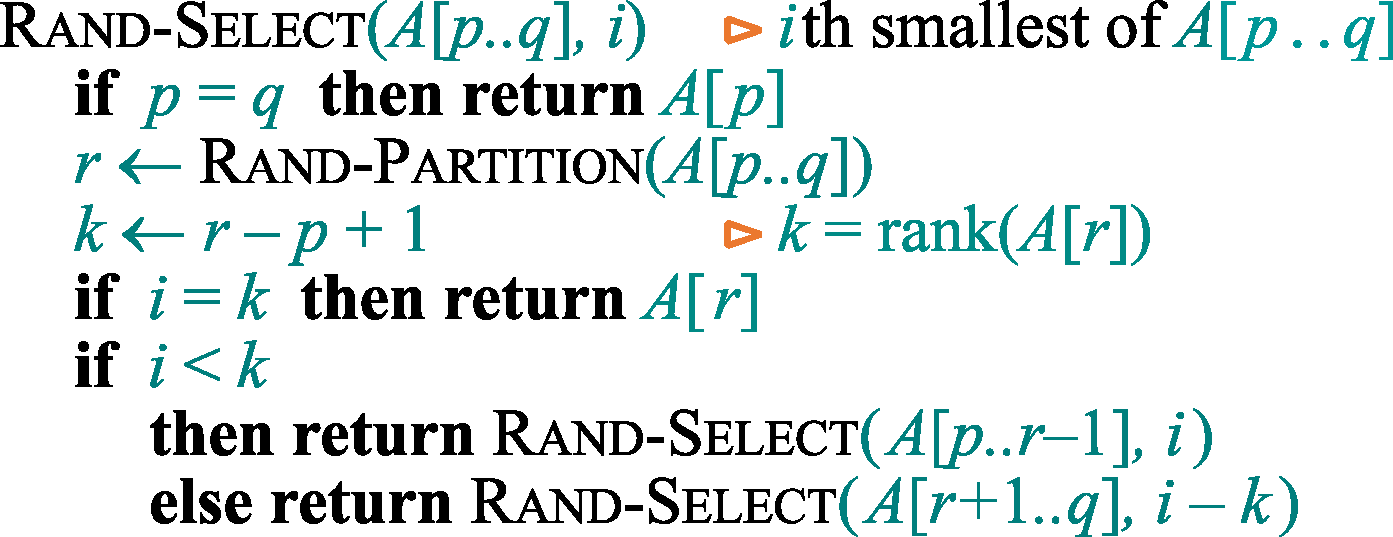
\includegraphics[width=\columnwidth]{rand-select.pdf}

\sldef{Median-of-medians}. Worst \(\Theta(n)\), but large constant.\\
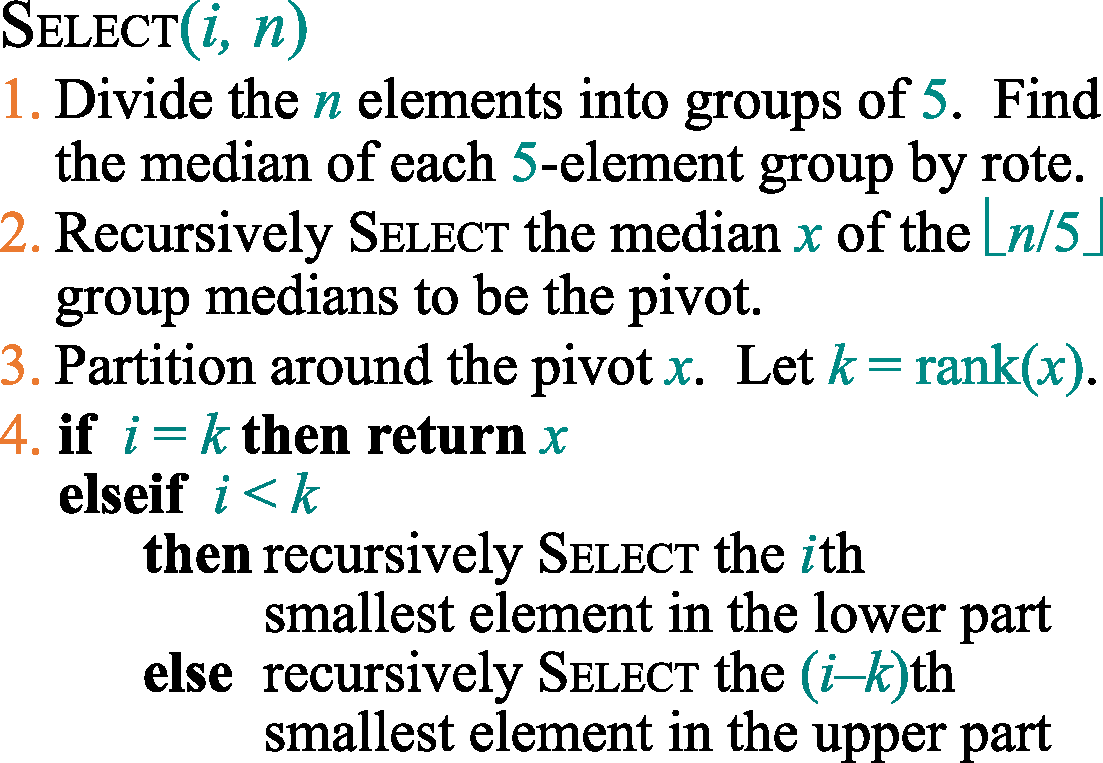
\includegraphics[width=0.8\columnwidth]{mom.pdf}
\end{document}
